% ============================================================
% Capítulo 7: Testes e Qualidade Automatizada
% ============================================================
\chapter{Testes e Qualidade Automatizada}

\section{Introdução}

Testes são a rede de segurança que permite que você mude código com confiança.
Sem testes, cada alteração é um salto no escuro. Com testes, cada alteração é
uma hipótese verificável.

\begin{itemize}
    \item \textbf{Testes como rede de segurança}: quando você refatora, adiciona
    funcionalidade ou corrige bugs, os testes garantem que o comportamento
    existente não foi quebrado. É o equivalente a escalar com corda --- você
    pode ousar mais porque a queda é controlada.
    \item \textbf{Testes como documentação executável}: um bom teste descreve
    exatamente o que o sistema faz. Diferente de um comentário, que pode ficar
    desatualizado, o teste falha quando a realidade muda. É a documentação que
    se autoatualiza.
    \item \textbf{Testes como feedback de design}: se é difícil testar uma função,
    o problema raramente é o teste --- é o design. Código com muitas dependências,
    estado global e efeitos colaterais escondidos é naturalmente resistente a
    testes. A dificuldade de testar é um sintoma, não a doença.
\end{itemize}

\subsection{O Custo dos Bugs em Cada Fase}

O custo de corrigir um bug cresce exponencialmente conforme ele avança no ciclo
de vida do software. Essa não é uma observação nova --- Barry Boehm documentou
isso nos anos 1980 --- mas continua sendo ignorada com frequência impressionante.

\begin{itemize}
    \item \textbf{Requisitos}: custo relativo \textbf{1x}. Corrigir um requisito
    mal escrito custa uma reunião.
    \item \textbf{Design}: custo relativo \textbf{5x}. Redesenhar uma arquitetura
    custa dias de trabalho e afeta múltiplos componentes.
    \item \textbf{Codificação}: custo relativo \textbf{10x}. Corrigir código já
    integrado exige entender dependências e regressões.
    \item \textbf{Teste}: custo relativo \textbf{20x}. Descobrir o bug aqui
    significa que ele já passou por revisão, integração e deploy em staging.
    \item \textbf{Produção}: custo relativo \textbf{100x ou mais}. Inclui impacto
    no usuário, perda de receita, dano à reputação, hotfixes emergenciais e
    noites sem dormir.
\end{itemize}

\subsection{Como a IA Muda o Panorama de Testes}

A IA generativa trouxe uma mudança real na prática de testes:

\begin{itemize}
    \item \textbf{Geração rápida de testes}: LLMs conseguem gerar dezenas de
    testes unitários em segundos, cobrindo caminhos que o desenvolvedor poderia
    esquecer.
    \item \textbf{Limitação fundamental}: a IA testa o que o código \textbf{faz},
    não o que ele \textbf{deveria fazer}. Ela não conhece seu domínio, suas
    regras de negócio, seus edge cases regulatórios. Ela replica padrões ---
    não valida intenções.
    \item \textbf{Novo papel do engenheiro}: o engenheiro deixa de ser quem
    escreve cada linha de teste e passa a ser quem \textbf{define a estratégia
    de teste}, revisa os testes gerados e garante que eles verificam o que
    realmente importa.
    \item \textbf{O teste como contrato com a IA}: no workflow TDD+IA, o
    engenheiro escreve o teste primeiro (definindo o comportamento esperado)
    e a IA implementa o código que satisfaz esse teste. O teste se torna a
    especificação executável que guia a geração.
\end{itemize}

% ============================================================
\section{Pirâmide de Testes Revisitada}
% ============================================================

A pirâmide de testes, popularizada por Mike Cohn, continua sendo um modelo
mental útil para distribuir o esforço de teste.

\begin{figure}[htbp]
    \centering
    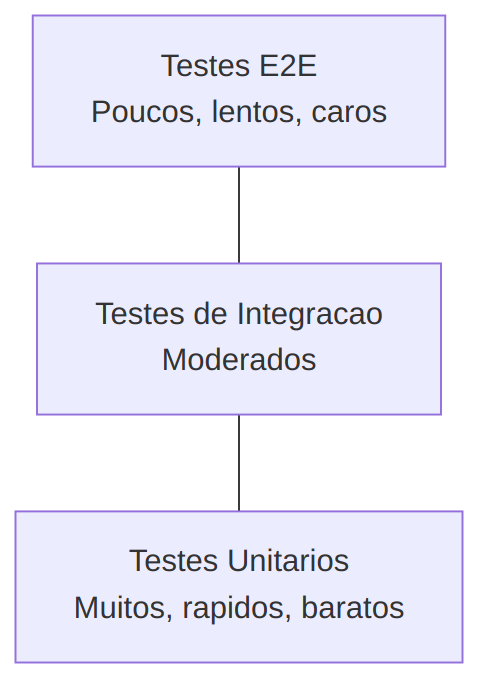
\includegraphics[width=0.85\textwidth]{imagens/07-testes-qualidade-automatizada-01-piramide-de-testes.png}
    \caption{Pirâmide de Testes}
\end{figure}

\subsection{Testes Unitários: A Base}

Testes unitários verificam uma unidade isolada de código --- tipicamente uma
função ou método --- sem dependências externas.

\begin{itemize}
    \item \textbf{Velocidade}: executam em milissegundos. Milhares deles rodam
    em segundos.
    \item \textbf{Isolamento}: não dependem de banco de dados, rede, sistema de
    arquivos ou outros serviços. Dependências são substituídas por doubles.
    \item \textbf{Quantidade}: devem compor 70--80\% da suíte de testes.
    \item \textbf{Custo}: baixo para escrever, baixo para manter, alto retorno
    em confiança.
    \item \textbf{Limitação}: não verificam se os componentes funcionam juntos.
    Cada peça pode passar individualmente e o sistema falhar na integração.
\end{itemize}

\begin{lstlisting}[language=Python, caption={Teste unitário com pytest}]
# calculadora.py
def calcular_desconto(preco: float, percentual: float) -> float:
    """Aplica desconto ao preco. Desconto maximo: 50%."""
    if preco < 0:
        raise ValueError("Preco nao pode ser negativo")
    if percentual < 0 or percentual > 50:
        raise ValueError("Desconto deve estar entre 0 e 50%")
    return round(preco * (1 - percentual / 100), 2)

# test_calculadora.py
import pytest
from calculadora import calcular_desconto

def test_desconto_basico():
    assert calcular_desconto(100.0, 10) == 90.0

def test_desconto_zero():
    assert calcular_desconto(100.0, 0) == 100.0

def test_desconto_maximo():
    assert calcular_desconto(100.0, 50) == 50.0

def test_preco_negativo_levanta_erro():
    with pytest.raises(ValueError, match="Preco nao pode ser negativo"):
        calcular_desconto(-10.0, 10)

def test_desconto_acima_do_maximo():
    with pytest.raises(ValueError, match="Desconto deve estar entre"):
        calcular_desconto(100.0, 60)

def test_desconto_com_centavos():
    assert calcular_desconto(99.99, 15) == 84.99
\end{lstlisting}

\subsection{Testes de Integração: O Meio}

Testes de integração verificam se dois ou mais componentes funcionam corretamente
juntos. O ``componente'' pode ser seu código com um banco de dados, uma API
externa, um sistema de filas ou outro microserviço.

\begin{itemize}
    \item \textbf{Velocidade}: mais lentos que unitários (segundos a minutos),
    pois envolvem I/O real.
    \item \textbf{Escopo}: verificam contratos entre componentes, serialização,
    queries SQL reais, chamadas HTTP.
    \item \textbf{Quantidade}: 15--20\% da suíte de testes.
    \item \textbf{Custo}: moderado. Exigem infraestrutura (bancos, containers)
    e são mais frágeis que unitários.
    \item \textbf{Valor}: capturam bugs que testes unitários nunca encontrariam
    --- o tipo de bug que aparece quando ``cada peça funciona sozinha mas o
    sistema não funciona junto''.
\end{itemize}

\subsection{Testes End-to-End (E2E): O Topo}

Testes E2E simulam o comportamento real do usuário, percorrendo fluxos completos
do sistema --- do clique no botão até a resposta na tela.

\begin{itemize}
    \item \textbf{Velocidade}: lentos (segundos a minutos por teste). Envolvem
    browser, rede, banco de dados, serviços externos.
    \item \textbf{Escopo}: verificam fluxos de negócio completos.
    \item \textbf{Quantidade}: 5--10\% da suíte. Poucos, mas estratégicos.
    \item \textbf{Custo}: alto para escrever, alto para manter, frequentemente
    flaky (falham intermitentemente).
    \item \textbf{Valor}: são os únicos que garantem que o sistema funciona do
    ponto de vista do usuário.
\end{itemize}

\subsection{Testes de Contrato}

Testes de contrato verificam que a interface entre dois serviços (produtor e
consumidor) respeita um acordo formal. São especialmente importantes em
arquiteturas de microserviços.

\begin{itemize}
    \item \textbf{Consumer-Driven Contracts}: o consumidor define o que espera
    da API. O produtor verifica que atende a essas expectativas. Ferramentas
    como \textbf{Pact} automatizam esse fluxo.
    \item \textbf{Vantagem}: detectam quebras de contrato antes do deploy, sem
    precisar rodar os dois serviços juntos.
    \item \textbf{Posição na pirâmide}: ficam entre integração e E2E. São mais
    rápidos que E2E, mas verificam interações reais entre serviços.
\end{itemize}

\subsection{A Pirâmide vs. O Troféu de Testes}

Kent C. Dodds propôs o \textit{Testing Trophy} como alternativa à pirâmide,
argumentando que testes de integração oferecem o melhor custo-benefício.

\begin{itemize}
    \item \textbf{Pirâmide}: muitos unitários, poucos E2E. Otimiza para
    velocidade e isolamento.
    \item \textbf{Troféu}: mais integração, menos unitários. Otimiza para
    confiança de que o sistema funciona como um todo.
    \item \textbf{Na prática}: a escolha depende do contexto. Sistemas com lógica
    de negócio complexa se beneficiam de muitos unitários. Sistemas com muitas
    integrações se beneficiam de mais testes de integração.
    \item \textbf{O erro}: o erro não é escolher pirâmide ou troféu. O erro é
    não ter estratégia nenhuma e testar aleatoriamente.
\end{itemize}

\subsection{Proporções e Custos}

\begin{table}[htbp]
\centering
\caption{Tipos de Teste: Comparação}
\begin{tabular}{@{}lllll@{}}
\toprule
\textbf{Tipo} & \textbf{Velocidade} & \textbf{Escopo} & \textbf{Custo} & \textbf{Quando usar} \\
\midrule
Unitário & ms & Função/classe & Baixo & Lógica de negócio, algoritmos \\
Integração & s & Componentes & Médio & Banco, APIs, filas \\
Contrato & s & Interface & Médio & Microserviços, APIs públicas \\
E2E & min & Sistema & Alto & Fluxos críticos de negócio \\
Performance & min--h & Sistema & Alto & Antes de releases, SLAs \\
\bottomrule
\end{tabular}
\end{table}

% ============================================================
\section{Test-Driven Development (TDD)}
% ============================================================

TDD não é uma técnica de teste. TDD é uma \textbf{técnica de design} que usa
testes como veículo. Essa distinção é fundamental.

\subsection{O Ciclo Red-Green-Refactor}

\begin{figure}[htbp]
    \centering
    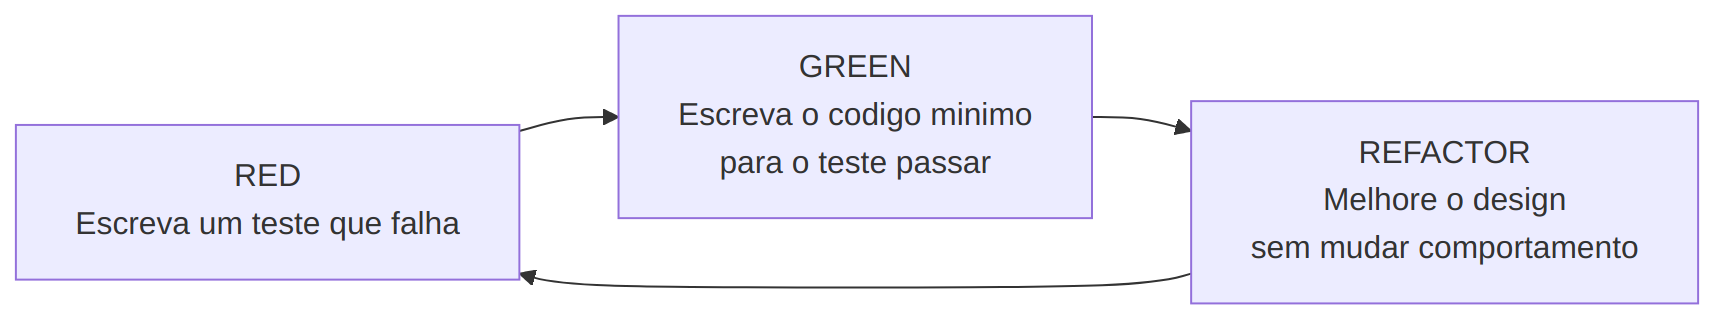
\includegraphics[width=0.85\textwidth]{imagens/07-testes-qualidade-automatizada-02-ciclo-tdd.png}
    \caption{Ciclo TDD}
\end{figure}

\begin{enumerate}
    \item \textbf{Red}: escreva um teste que descreve o comportamento desejado.
    Execute-o. Ele deve falhar. Se não falhar, o teste não está testando nada
    novo.
    \item \textbf{Green}: escreva o código \textbf{mínimo} para fazer o teste
    passar. Não antecipe. Não generalize. Não refatore. Apenas faça o teste
    ficar verde.
    \item \textbf{Refactor}: agora, com o teste verde como rede de segurança,
    melhore o design. Remova duplicação, extraia funções, renomeie variáveis.
    O teste garante que você não quebrou nada.
\end{enumerate}

\subsection{TDD como Técnica de Design}

O valor do TDD não está nos testes que ele produz --- está nas decisões de
design que ele força:

\begin{itemize}
    \item \textbf{Foco no comportamento}: ao escrever o teste primeiro, você
    define \textit{o que} o código deve fazer antes de pensar em \textit{como}.
    Isso produz interfaces mais claras.
    \item \textbf{Feedback imediato}: cada ciclo leva minutos. Você descobre
    problemas de design rapidamente, não depois de 500 linhas escritas.
    \item \textbf{Escopo controlado}: a disciplina de implementar apenas o
    mínimo evita over-engineering. Você constrói apenas o que o teste exige.
    \item \textbf{Refatoração segura}: com testes passando, você pode
    reestruturar o código sabendo que o comportamento está preservado.
\end{itemize}

\subsection{Quando TDD Vale a Pena --- e Quando Não}

TDD não é dogma. É ferramenta. Use quando faz sentido.

\begin{itemize}
    \item \textbf{Vale a pena}: lógica de negócio complexa, algoritmos com muitos
    edge cases, código que será mantido por longo tempo, APIs públicas.
    \item \textbf{Talvez não valha}: protótipos descartáveis, scripts de uso
    único, código de UI altamente visual (onde o feedback é visual, não lógico),
    exploração inicial de um domínio desconhecido.
    \item \textbf{Regra prática}: se o código vai durar mais de uma semana e tem
    lógica que pode quebrar, TDD compensa. Se é descartável, escreva o teste
    depois --- ou não escreva.
\end{itemize}

\subsection{TDD + IA: O Workflow do Capítulo 4}

A combinação de TDD com IA cria um workflow poderoso:

\begin{enumerate}
    \item \textbf{Engenheiro escreve o teste}: define o comportamento esperado,
    os edge cases, as pré-condições e pós-condições. Isso exige conhecimento
    do domínio --- algo que a IA não tem.
    \item \textbf{IA implementa o código}: dado o teste como especificação, a
    IA gera o código que o satisfaz. O teste funciona como um contrato
    verificável.
    \item \textbf{Engenheiro revisa e refatora}: verifica se a implementação é
    correta, eficiente e legível. Refatora com segurança, pois os testes
    garantem o comportamento.
\end{enumerate}

Nesse modelo, o teste é a \textbf{língua franca} entre humano e IA. O humano
expressa intenção via teste; a IA traduz essa intenção em código.

\subsection{Walkthrough Completo: Calculadora de Descontos com TDD}

Vamos construir uma calculadora de descontos progressivos usando TDD rigoroso.
Cada ciclo mostra Red, Green e Refactor.

\textbf{Regra de negócio}: descontos são progressivos por faixa de valor.
Compras até R\$100 não têm desconto. De R\$100 a R\$500, desconto de 5\%.
Acima de R\$500, desconto de 10\%.

\subsubsection{Ciclo 1: Sem desconto para valores baixos}

\begin{lstlisting}[language=Python, caption={Ciclo 1 --- Red: teste para valor sem desconto}]
# test_desconto_progressivo.py
from desconto_progressivo import calcular_desconto_progressivo

def test_sem_desconto_para_valores_ate_100():
    assert calcular_desconto_progressivo(50.0) == 50.0
    assert calcular_desconto_progressivo(100.0) == 100.0
\end{lstlisting}

\begin{lstlisting}[language=Python, caption={Ciclo 1 --- Green: implementação mínima}]
# desconto_progressivo.py
def calcular_desconto_progressivo(valor: float) -> float:
    return valor
\end{lstlisting}

Nenhuma refatoração necessária --- o código é trivial. Seguimos.

\subsubsection{Ciclo 2: Desconto de 5\% para faixa intermediária}

\begin{lstlisting}[language=Python, caption={Ciclo 2 --- Red: teste para faixa intermediária}]
def test_desconto_5_porcento_entre_100_e_500():
    assert calcular_desconto_progressivo(200.0) == 190.0
    assert calcular_desconto_progressivo(500.0) == 475.0
\end{lstlisting}

\begin{lstlisting}[language=Python, caption={Ciclo 2 --- Green: adicionando a primeira faixa}]
def calcular_desconto_progressivo(valor: float) -> float:
    if valor > 100:
        return round(valor * 0.95, 2)
    return valor
\end{lstlisting}

\subsubsection{Ciclo 3: Desconto de 10\% para valores altos}

\begin{lstlisting}[language=Python, caption={Ciclo 3 --- Red: teste para faixa alta}]
def test_desconto_10_porcento_acima_de_500():
    assert calcular_desconto_progressivo(1000.0) == 900.0
    assert calcular_desconto_progressivo(500.01) == 450.01
\end{lstlisting}

\begin{lstlisting}[language=Python, caption={Ciclo 3 --- Green: implementação completa}]
def calcular_desconto_progressivo(valor: float) -> float:
    if valor > 500:
        return round(valor * 0.90, 2)
    if valor > 100:
        return round(valor * 0.95, 2)
    return valor
\end{lstlisting}

\begin{lstlisting}[language=Python, caption={Ciclo 3 --- Refactor: extraindo as faixas}]
from typing import List, Tuple

# Faixas: (limite_minimo, percentual_desconto)
FAIXAS_DESCONTO: List[Tuple[float, float]] = [
    (500.0, 10.0),
    (100.0, 5.0),
    (0.0, 0.0),
]

def calcular_desconto_progressivo(valor: float) -> float:
    """Calcula desconto progressivo por faixa de valor."""
    if valor < 0:
        raise ValueError("Valor nao pode ser negativo")
    for limite, desconto in FAIXAS_DESCONTO:
        if valor > limite:
            return round(valor * (1 - desconto / 100), 2)
    return valor
\end{lstlisting}

Observe: após a refatoração, todos os testes anteriores continuam passando. As
faixas agora são dados configuráveis, não lógica hardcoded. Se uma nova faixa
surgir, basta adicionar uma tupla à lista.

% ============================================================
\section{Testes com Assistência de IA}
% ============================================================

\subsection{O Que a IA Faz Bem}

\begin{itemize}
    \item \textbf{Gerar testes para caminhos óbvios}: dado um código existente,
    a IA identifica caminhos felizes, edge cases comuns e exceções esperadas
    com velocidade impressionante.
    \item \textbf{Boilerplate de testes}: setup, teardown, fixtures, mocks ---
    a IA gera a infraestrutura de teste rapidamente.
    \item \textbf{Testes de regressão}: ao receber um bug report, a IA pode
    gerar um teste que reproduz o bug antes da correção.
    \item \textbf{Cobertura de branches}: a IA analisa o código e gera testes
    para cada branch de execução, aumentando a cobertura mecânica.
\end{itemize}

\subsection{O Que a IA Não Faz}

\begin{itemize}
    \item \textbf{Validar intenção}: a IA não sabe se o código \textit{deveria}
    retornar 42 ou 43. Ela testa que ele retorna o que retorna.
    \item \textbf{Entender regras de negócio}: ``cliente VIP não paga frete acima
    de R\$200'' é uma regra que a IA não infere do código.
    \item \textbf{Priorizar o que testar}: a IA trata todos os caminhos
    igualmente. O engenheiro sabe que o cálculo de juros é mais crítico que a
    formatação de data.
    \item \textbf{Testar o que não existe}: a IA não gera testes para
    funcionalidades que deveriam existir mas não foram implementadas.
\end{itemize}

\textbf{Regra de ouro}: a IA testa o que \textbf{É}. O engenheiro testa o que
\textbf{DEVERIA SER}.

\subsection{Testes Baseados em Propriedades com IA}

Testes baseados em propriedades (\textit{property-based testing}) verificam que
uma propriedade invariante vale para qualquer entrada válida, não apenas para
exemplos específicos.

\begin{lstlisting}[language=Python, caption={Teste baseado em propriedades com Hypothesis}]
from hypothesis import given, strategies as st
from desconto_progressivo import calcular_desconto_progressivo

@given(valor=st.floats(min_value=0.01, max_value=100_000.0))
def test_desconto_nunca_retorna_valor_negativo(valor):
    resultado = calcular_desconto_progressivo(valor)
    assert resultado >= 0

@given(valor=st.floats(min_value=0.01, max_value=100_000.0))
def test_desconto_nunca_excede_valor_original(valor):
    resultado = calcular_desconto_progressivo(valor)
    assert resultado <= valor

@given(valor=st.floats(min_value=500.01, max_value=100_000.0))
def test_faixa_alta_tem_desconto_maior_que_faixa_media(valor):
    resultado = calcular_desconto_progressivo(valor)
    # 10% de desconto significa que resultado = 90% do valor
    assert resultado == round(valor * 0.90, 2)
\end{lstlisting}

A IA pode ajudar a identificar propriedades candidatas analisando o código, mas
o engenheiro precisa validar se essas propriedades refletem regras reais do
domínio.

\subsection{Geração de Dados de Teste}

A IA é excelente para gerar dados de teste realistas:

\begin{itemize}
    \item \textbf{Fixtures complexas}: objetos com muitos campos e relações.
    \item \textbf{Dados limítrofes}: valores no limite exato de faixas, strings
    com caracteres especiais, datas em anos bissextos.
    \item \textbf{Combinações}: a IA pode gerar matrizes de combinação
    (pairwise testing) que cobrirão interações entre parâmetros.
    \item \textbf{Dados anônimos}: substituir dados reais por dados fictícios
    que preservam as características estatísticas.
\end{itemize}

\subsection{Análise de Cobertura}

Cobertura de código é uma métrica necessária, mas insuficiente.

\begin{itemize}
    \item \textbf{100\% de cobertura não significa 100\% de qualidade}: você pode
    cobrir todas as linhas sem verificar nada útil (\texttt{assert True}).
    \item \textbf{Cobertura como piso, não como teto}: defina um mínimo (ex.:
    80\%) e concentre-se na qualidade dos testes, não no número.
    \item \textbf{A IA e a armadilha da cobertura}: LLMs conseguem gerar testes
    que aumentam cobertura rapidamente, mas muitos desses testes são
    \textit{tautológicos} --- verificam que o código faz o que faz, sem
    questionar se deveria.
\end{itemize}

\subsection{Comparação: Teste Gerado por IA vs. Teste Escrito por Humano}

\begin{lstlisting}[language=Python, caption={Teste gerado por IA (tipicamente)}]
# IA gera testes mecanicos baseados no codigo existente
def test_calcular_desconto_progressivo_com_200():
    resultado = calcular_desconto_progressivo(200.0)
    assert resultado == 190.0  # Verifica o que o codigo retorna

def test_calcular_desconto_progressivo_com_1000():
    resultado = calcular_desconto_progressivo(1000.0)
    assert resultado == 900.0  # Verifica o que o codigo retorna
\end{lstlisting}

\begin{lstlisting}[language=Python, caption={Teste escrito por humano (idealmente)}]
# Humano testa regras de negocio e edge cases criticos
def test_limite_exato_da_faixa_nao_recebe_desconto():
    """R$100 exatos nao devem ter desconto (regra: acima de R$100)."""
    assert calcular_desconto_progressivo(100.0) == 100.0

def test_um_centavo_acima_do_limite_recebe_desconto():
    """R$100.01 ja entra na faixa de 5%."""
    assert calcular_desconto_progressivo(100.01) == 95.01

def test_transicao_entre_faixas():
    """R$500 esta na faixa de 5%. R$500.01 esta na faixa de 10%."""
    assert calcular_desconto_progressivo(500.0) == 475.0
    assert calcular_desconto_progressivo(500.01) == 450.01
\end{lstlisting}

A diferença é sutil mas crucial: o teste humano expressa \textbf{intenção de
negócio}, não apenas verificação mecânica. O nome do teste, o docstring e os
valores escolhidos comunicam \textit{por que} esse caso importa.

% ============================================================
\section{Testes de Integração e E2E}
% ============================================================

\subsection{Test Doubles: Mocks, Stubs, Fakes e Spies}

Test doubles são substitutos para dependências reais durante testes. Cada tipo
tem um propósito específico.

\begin{figure}[htbp]
    \centering
    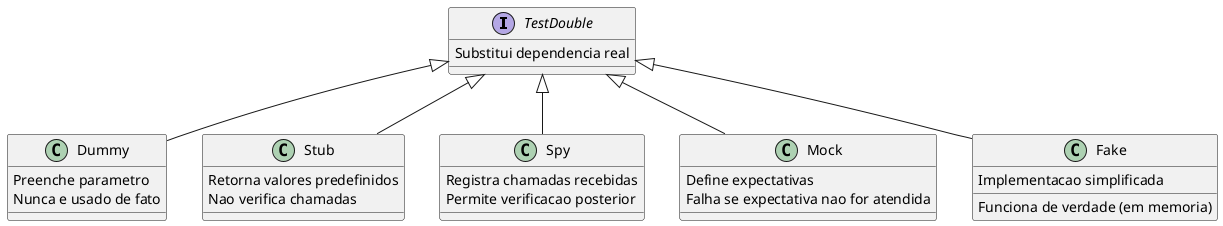
\includegraphics[width=0.85\textwidth]{imagens/07-testes-qualidade-automatizada-03-hierarquia-de-test-doubles.png}
    \caption{Hierarquia de Test Doubles}
\end{figure}

\begin{table}[htbp]
\centering
\caption{Test Doubles: Quando Usar Cada Um}
\begin{tabular}{@{}llll@{}}
\toprule
\textbf{Tipo} & \textbf{O que faz} & \textbf{Quando usar} & \textbf{Exemplo} \\
\midrule
Dummy & Preenche parâmetro & Parâmetro obrigatório não usado & Objeto vazio \\
Stub & Retorno fixo & Isolar dependência & API retorna JSON fixo \\
Spy & Registra chamadas & Verificar interação & Email foi enviado? \\
Mock & Expectativa rígida & Verificar contrato & Método X chamado 2x \\
Fake & Implementação real & Teste mais realista & Banco em memória \\
\bottomrule
\end{tabular}
\end{table}

\subsection{Mock vs. Fake: Comparação em Código}

\begin{lstlisting}[language=Python, caption={Usando Mock: verifica interação}]
from unittest.mock import Mock

def test_servico_envia_email_ao_criar_pedido():
    email_service = Mock()
    servico = ServicoDePedido(email_service=email_service)

    servico.criar_pedido(cliente_id=1, itens=["item1"])

    # Verifica que o metodo foi chamado com argumentos esperados
    email_service.enviar.assert_called_once_with(
        destinatario="cliente@email.com",
        assunto="Pedido confirmado"
    )
\end{lstlisting}

\begin{lstlisting}[language=Python, caption={Usando Fake: implementação simplificada}]
class FakeRepositorioDePedidos:
    """Repositorio em memoria para testes."""
    def __init__(self):
        self.pedidos = {}
        self._proximo_id = 1

    def salvar(self, pedido):
        pedido.id = self._proximo_id
        self.pedidos[pedido.id] = pedido
        self._proximo_id += 1
        return pedido

    def buscar_por_id(self, pedido_id):
        return self.pedidos.get(pedido_id)

def test_criar_pedido_persiste_no_repositorio():
    repo = FakeRepositorioDePedidos()
    servico = ServicoDePedido(repositorio=repo)

    pedido = servico.criar_pedido(cliente_id=1, itens=["item1"])

    assert repo.buscar_por_id(pedido.id) is not None
    assert repo.buscar_por_id(pedido.id).itens == ["item1"]
\end{lstlisting}

\textbf{Quando usar Mock}: quando você quer verificar \textit{que} uma
interação aconteceu (ex.: email foi enviado, evento foi publicado).

\textbf{Quando usar Fake}: quando você quer verificar \textit{o resultado}
de uma operação que depende de infraestrutura (ex.: dados foram persistidos,
cache foi atualizado).

\subsection{Testcontainers: Ambientes Efêmeros}

Testcontainers permite subir containers Docker durante o teste e destruí-los
ao final. O resultado são testes de integração que usam infraestrutura real,
mas são isolados e reproduzíveis.

\begin{lstlisting}[language=Python, caption={Teste de integração com Testcontainers}]
import pytest
from testcontainers.postgres import PostgresContainer
from sqlalchemy import create_engine, text

@pytest.fixture(scope="module")
def postgres_engine():
    with PostgresContainer("postgres:16") as postgres:
        engine = create_engine(postgres.get_connection_url())
        # Executa migrations
        with engine.connect() as conn:
            conn.execute(text("""
                CREATE TABLE pedidos (
                    id SERIAL PRIMARY KEY,
                    cliente_id INTEGER NOT NULL,
                    valor DECIMAL(10,2) NOT NULL,
                    status VARCHAR(20) DEFAULT 'pendente'
                )
            """))
            conn.commit()
        yield engine
        # Container e destruido automaticamente ao sair do with

def test_inserir_e_buscar_pedido(postgres_engine):
    with postgres_engine.connect() as conn:
        conn.execute(text(
            "INSERT INTO pedidos (cliente_id, valor) VALUES (1, 150.00)"
        ))
        conn.commit()

        resultado = conn.execute(text(
            "SELECT valor, status FROM pedidos WHERE cliente_id = 1"
        )).fetchone()

    assert resultado.valor == 150.00
    assert resultado.status == "pendente"
\end{lstlisting}

\begin{itemize}
    \item \textbf{Vantagem}: testa contra banco de dados real (PostgreSQL, MySQL,
    Redis, MongoDB), não contra mocks.
    \item \textbf{Isolamento}: cada execução começa com um container limpo.
    \item \textbf{CI/CD}: funciona em qualquer pipeline que tenha Docker.
    \item \textbf{Custo}: containers levam segundos para iniciar. Aceitável para
    integração, inaceitável para unitários.
\end{itemize}

\subsection{Testes de API e Contrato}

\begin{itemize}
    \item \textbf{Pact}: framework de Consumer-Driven Contracts. O consumidor
    define o contrato (``espero que GET /usuarios/1 retorne nome e email''),
    e o produtor verifica que atende.
    \item \textbf{Schema validation}: validar que a resposta da API corresponde
    ao schema OpenAPI/JSON Schema esperado.
    \item \textbf{Snapshot testing}: capturar a resposta da API e comparar com
    um snapshot salvo. Útil para detectar mudanças inesperadas.
\end{itemize}

\subsection{E2E com Playwright e Cypress}

\begin{itemize}
    \item \textbf{Playwright}: suporte a múltiplos browsers (Chromium, Firefox,
    WebKit), API moderna em Python/JS/Java/.NET, excelente para testes
    cross-browser.
    \item \textbf{Cypress}: excelente developer experience, execução no browser,
    time-travel debugging. Limitado a Chromium-based browsers.
    \item \textbf{IA na criação de E2E}: LLMs podem gerar scripts de E2E a
    partir de descrições em linguagem natural (``teste o fluxo de checkout:
    adicionar item ao carrinho, ir para pagamento, preencher dados, confirmar
    pedido''). O resultado é um bom ponto de partida, mas quase sempre requer
    ajustes para seletores, waits e assertions específicas.
\end{itemize}

% ============================================================
\section{Testes de Performance e Carga}
% ============================================================

Testes de performance respondem a uma pergunta que testes funcionais não fazem:
``o sistema funciona \textbf{rápido o suficiente} sob \textbf{carga realista}?''

\subsection{Por Que Testes de Performance Importam}

\begin{itemize}
    \item \textbf{Caso real: Black Friday}: um e-commerce que nunca testou carga
    caiu nos primeiros 5 minutos de promoção. A correção custou milhões em
    perda de vendas e reputação.
    \item \textbf{Caso real: Latência crescente}: um microsserviço que levava
    50ms para responder passou a levar 2s após uma mudança aparentemente
    inofensiva no ORM. Sem teste de performance, o problema foi detectado em
    produção.
    \item \textbf{SLAs}: se o contrato com o cliente exige 99.9\% de
    disponibilidade e latência p95 abaixo de 200ms, você precisa provar
    isso com testes, não com esperança.
\end{itemize}

\subsection{Ferramentas}

\begin{table}[htbp]
\centering
\caption{Ferramentas de Teste por Linguagem e Propósito}
\begin{tabular}{@{}llll@{}}
\toprule
\textbf{Ferramenta} & \textbf{Linguagem} & \textbf{Propósito} & \textbf{Destaque} \\
\midrule
pytest & Python & Unitário/Integração & Fixtures, plugins \\
unittest & Python & Unitário & Padrão da stdlib \\
Hypothesis & Python & Property-based & Geração automática de dados \\
JUnit 5 & Java & Unitário/Integração & Extensões, parametrização \\
Jest & JavaScript & Unitário/Integração & Snapshots, mocks \\
Playwright & Multi & E2E & Cross-browser, multi-linguagem \\
Cypress & JavaScript & E2E & DX excelente, time-travel \\
k6 & JavaScript & Performance & Scripting em JS, métricas ricas \\
Gatling & Scala/Java & Performance & DSL expressiva, relatórios \\
Locust & Python & Performance & Código Python, distribuído \\
Pact & Multi & Contrato & Consumer-driven contracts \\
Testcontainers & Multi & Integração & Containers efêmeros \\
\bottomrule
\end{tabular}
\end{table}

\subsection{IA Gerando Cenários de Carga}

A IA pode ajudar a gerar cenários de carga a partir de descrições de uso:

\begin{itemize}
    \item \textbf{Traduzir métricas de produção}: ``temos 10.000 usuários
    simultâneos com 60\% de reads e 40\% de writes'' se transforma em um
    script k6 ou Locust com os ratios corretos.
    \item \textbf{Gerar dados variados}: distribuições realistas de tamanhos
    de payload, tempos de think-time entre requisições, padrões de acesso.
    \item \textbf{Limitação}: a IA não sabe quais cenários são relevantes para
    \textit{seu} sistema. ``O que acontece quando 5.000 usuários tentam
    comprar o mesmo produto ao mesmo tempo?'' é uma pergunta que exige
    conhecimento do domínio.
\end{itemize}

\subsection{Métricas e Interpretação}

\begin{itemize}
    \item \textbf{Latência}: p50 (mediana), p95, p99. A média mente --- use
    percentis. Se o p50 é 50ms mas o p99 é 5s, 1\% dos seus usuários está
    tendo uma experiência péssima.
    \item \textbf{Throughput}: requisições por segundo que o sistema sustenta
    antes de degradar.
    \item \textbf{Taxa de erros}: percentual de requisições que falham sob carga.
    Deve ser zero (ou próximo) até o limite de capacidade.
    \item \textbf{Saturação}: CPU, memória, conexões de banco, threads.
    Identifica o gargalo antes que ele cause falhas.
    \item \textbf{Análise prática}: rode testes com carga crescente (ramp-up).
    Identifique o ponto de inflexão onde a latência começa a crescer
    exponencialmente. Esse é o limite real do seu sistema.
\end{itemize}

% ============================================================
\section{Mutation Testing e Qualidade de Testes}
% ============================================================

Cobertura de código mede se o teste \textit{executa} o código. Mutation testing
mede se o teste \textit{detecta} mudanças no código. A diferença é enorme.

\subsection{O Que É Mutation Testing}

Mutation testing funciona assim:

\begin{enumerate}
    \item Uma ferramenta cria ``mutantes'' do código original --- pequenas
    alterações como trocar \texttt{>} por \texttt{>=}, \texttt{+} por
    \texttt{-}, \texttt{True} por \texttt{False}.
    \item Os testes existentes são executados contra cada mutante.
    \item Se um teste falha (detecta a mutação), o mutante é \textbf{morto}.
    Bom.
    \item Se nenhum teste falha (a mutação passou despercebida), o mutante
    \textbf{sobreviveu}. Isso indica uma lacuna nos testes.
\end{enumerate}

\begin{figure}[htbp]
    \centering
    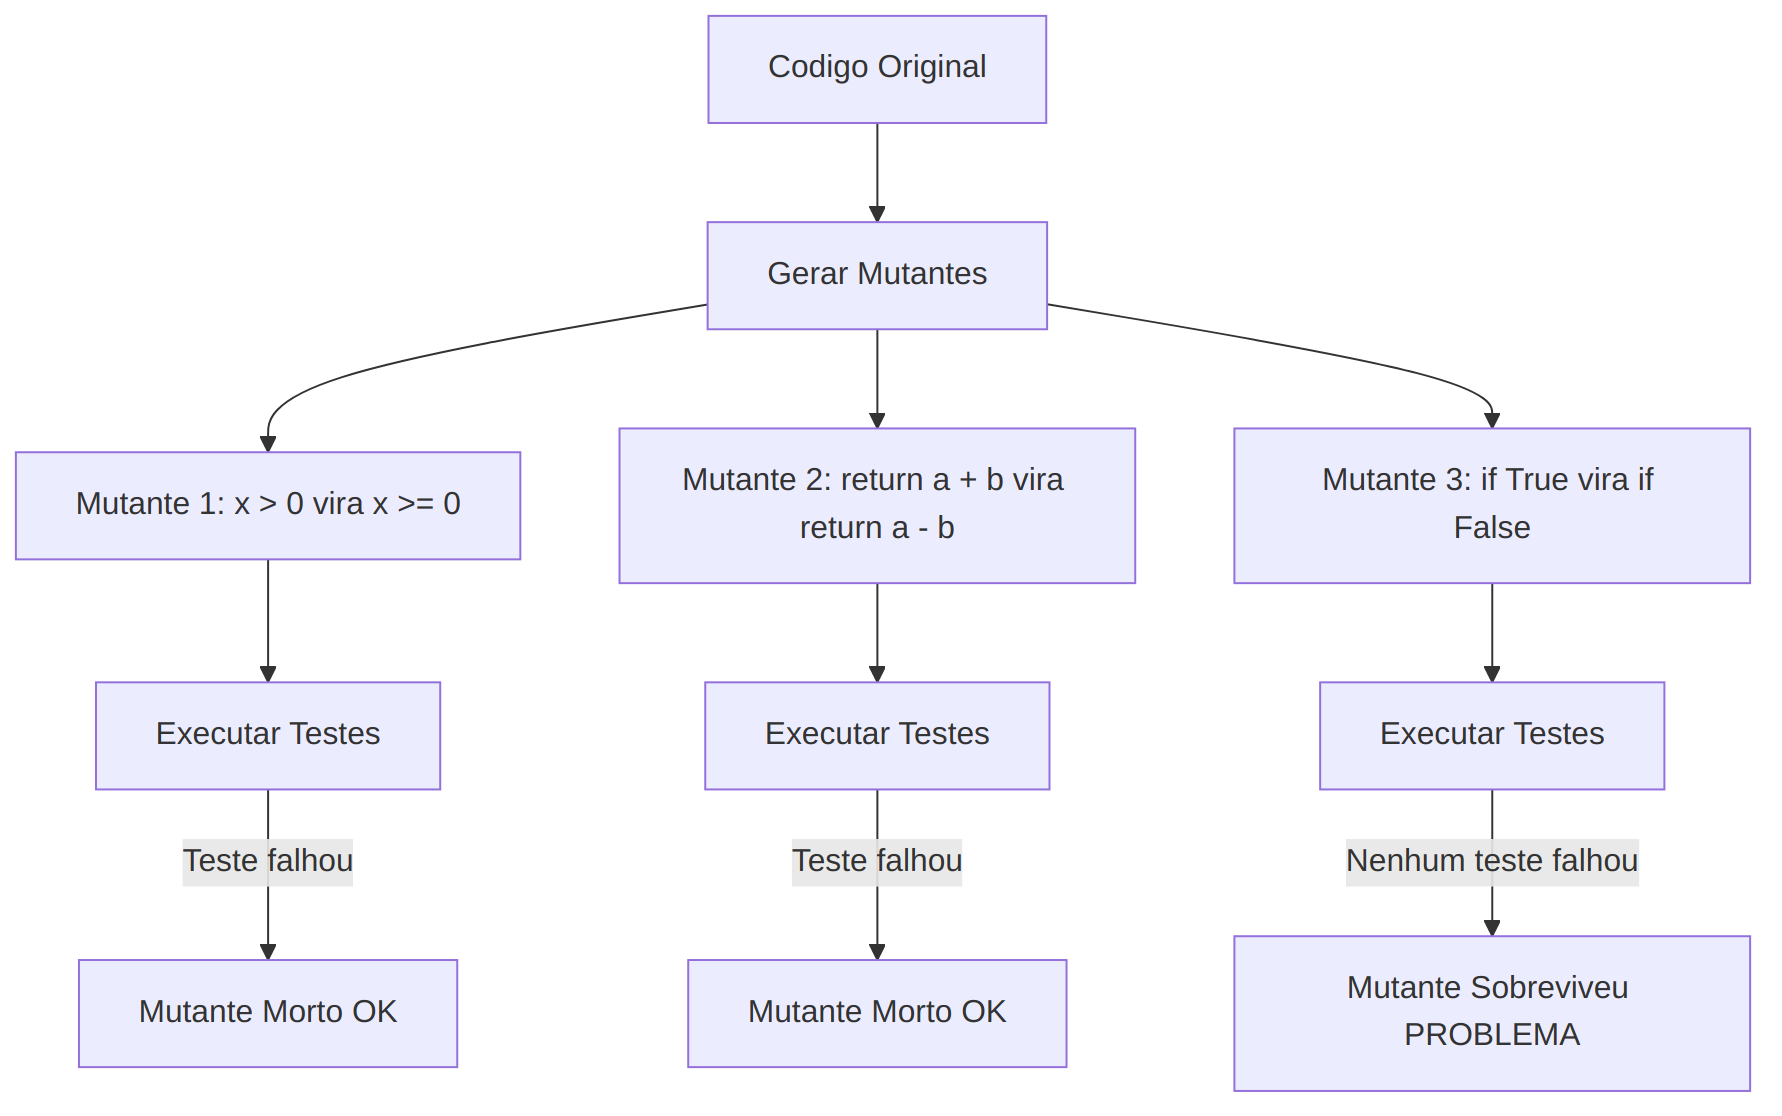
\includegraphics[width=0.85\textwidth]{imagens/07-testes-qualidade-automatizada-04-fluxo-de-mutation-testing.png}
    \caption{Fluxo de Mutation Testing}
\end{figure}

\subsection{Ferramentas de Mutation Testing}

\begin{itemize}
    \item \textbf{PIT} (Java): o mais maduro do ecossistema Java. Integra com
    Maven/Gradle, suporte a JUnit e TestNG.
    \item \textbf{mutmut} (Python): mutation testing para Python. Simples de
    configurar, funciona com pytest.
    \item \textbf{Stryker} (JavaScript/TypeScript): suporte a Jest, Mocha,
    Karma. Dashboard web com relatórios visuais.
    \item \textbf{Cosmic Ray} (Python): alternativa ao mutmut com suporte a
    execução distribuída.
\end{itemize}

\subsection{Mutation Score vs. Code Coverage}

\begin{itemize}
    \item \textbf{Code coverage}: ``90\% das linhas foram executadas pelos
    testes.'' Não diz nada sobre a qualidade das assertions.
    \item \textbf{Mutation score}: ``85\% dos mutantes foram detectados pelos
    testes.'' Mede diretamente se os testes verificam o comportamento, não
    apenas se o código é executado.
    \item \textbf{Exemplo}: um teste que chama uma função mas não faz nenhum
    \texttt{assert} contribui para cobertura, mas não mata nenhum mutante.
    \item \textbf{Na prática}: mutation score abaixo de 60\% indica testes
    fracos, mesmo com cobertura alta. Acima de 80\% é considerado bom.
\end{itemize}

\subsection{Quando Mutation Testing Vale o Custo}

Mutation testing é computacionalmente caro: cada mutante requer uma execução
completa dos testes.

\begin{itemize}
    \item \textbf{Vale a pena}: código crítico (financeiro, saúde, segurança),
    bibliotecas públicas, domínios onde bugs têm custo altíssimo.
    \item \textbf{Talvez não valha}: código de prototipação, projetos pequenos
    com equipe única, código com baixa complexidade ciclomática.
    \item \textbf{Estratégia prática}: não rode mutation testing em todo o
    código. Aplique nos módulos mais críticos. Use como auditoria periódica,
    não como gate em cada PR.
\end{itemize}

% ============================================================
\section{CI/CD e Pipeline de Testes}
% ============================================================

Um pipeline de testes bem desenhado segue um princípio simples: \textbf{feedback
rápido primeiro, validação profunda depois}.

\subsection{Estágios do Pipeline}

\begin{figure}[htbp]
    \centering
    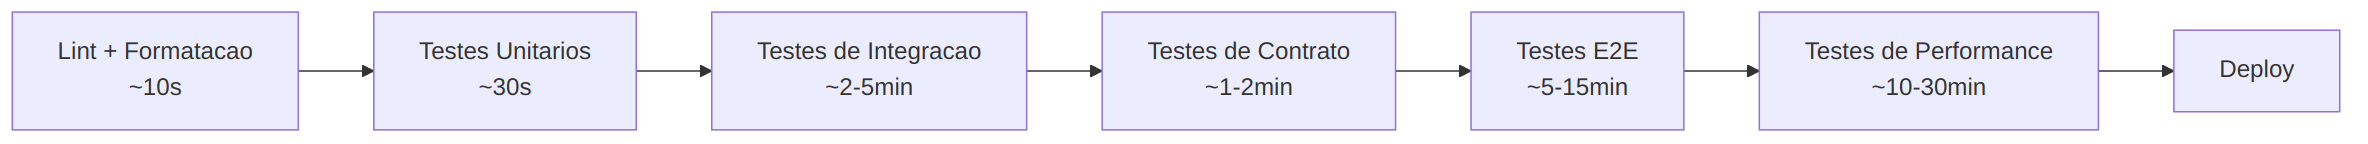
\includegraphics[width=0.85\textwidth]{imagens/07-testes-qualidade-automatizada-05-pipeline-de-testes-em-ci-cd.png}
    \caption{Pipeline de Testes em CI/CD}
\end{figure}

\begin{enumerate}
    \item \textbf{Lint e Formatação} (\textasciitilde10 segundos): verificação
    estática. Se o código não compila ou não está formatado, não faz sentido
    rodar testes.
    \item \textbf{Testes Unitários} (\textasciitilde30 segundos): a primeira
    linha de defesa. Rápidos, isolados, sem dependências externas.
    \item \textbf{Testes de Integração} (\textasciitilde2-5 minutos): verificam
    interação com banco, APIs, filas. Usam Testcontainers ou serviços efêmeros.
    \item \textbf{Testes de Contrato} (\textasciitilde1-2 minutos): verificam
    que as interfaces entre serviços não foram quebradas.
    \item \textbf{Testes E2E} (\textasciitilde5-15 minutos): verificam fluxos
    completos de negócio. Executados em ambiente que simula produção.
    \item \textbf{Testes de Performance} (\textasciitilde10-30 minutos):
    executados em releases ou branches específicas, não em cada PR.
\end{enumerate}

\subsection{Fast Feedback Loop}

\begin{itemize}
    \item \textbf{Regra dos 10 minutos}: se o desenvolvedor precisa esperar
    mais de 10 minutos para saber se seu código está correto, algo está
    errado no pipeline.
    \item \textbf{Paralelização}: testes unitários e lint rodam em paralelo.
    Testes de integração e contrato podem rodar em paralelo entre si.
    \item \textbf{Cache inteligente}: reutilizar imagens Docker, dependências
    instaladas, builds anteriores. A diferença entre um pipeline de 15 minutos
    e um de 3 minutos está frequentemente no cache.
    \item \textbf{Selective testing}: rodar apenas testes afetados pela mudança.
    Se você alterou o módulo de pagamento, não precisa rodar testes do módulo
    de relatórios.
\end{itemize}

\subsection{Quality Gates Antes do Merge}

Um quality gate é uma condição que deve ser satisfeita antes que o código
seja integrado ao branch principal.

\begin{itemize}
    \item \textbf{Todos os testes passam}: condição óbvia, frequentemente
    violada por pressão de prazo.
    \item \textbf{Cobertura mínima}: ex.: cobertura de novas linhas deve ser
    pelo menos 80\%. Não exija 100\% --- isso incentiva testes inúteis.
    \item \textbf{Análise estática}: sem warnings novos de linters, sem
    vulnerabilidades de segurança conhecidas.
    \item \textbf{Review aprovado}: pelo menos um reviewer humano aprovou.
    \item \textbf{Sem regressões de performance}: se aplicável, latência p95
    não piorou mais que 10\%.
\end{itemize}

\subsection{Testes Flaky: Detecção e Eliminação}

Testes flaky são aqueles que passam e falham intermitentemente sem mudança no
código. São o câncer de uma suíte de testes.

\begin{itemize}
    \item \textbf{Por que são perigosos}: destroem a confiança na suíte. Se os
    testes falham ``de vez em quando'', a equipe começa a ignorar falhas ---
    incluindo falhas reais.
    \item \textbf{Causas comuns}: dependência de tempo (\texttt{sleep},
    \texttt{time.now()}), ordem de execução, estado compartilhado entre testes,
    race conditions, dependência de rede.
    \item \textbf{Detecção}: rode a suíte de testes N vezes consecutivas sem
    mudança de código. Testes que falham em qualquer execução são candidatos.
    Ferramentas como \texttt{pytest-repeat} automatizam isso.
    \item \textbf{Eliminação}: isole o teste, identifique a dependência
    externa, substitua por determinismo. Relógio controlado em vez de
    \texttt{time.now()}, seeds fixas para aleatoriedade, setup/teardown
    isolados.
    \item \textbf{Quarentena}: se não pode corrigir imediatamente, mova o teste
    para uma suíte separada marcada como flaky. Não o delete --- corrija-o na
    próxima sprint.
\end{itemize}

\subsection{Fail Fast, Recover Faster}

\begin{itemize}
    \item \textbf{Fail fast}: estruture o pipeline para que falhas baratas
    (lint, unitários) ocorram antes de falhas caras (E2E, performance).
    Se um teste unitário falha em 30 segundos, você economiza os 15 minutos
    dos testes E2E.
    \item \textbf{Recover faster}: quando a build quebra, a prioridade da equipe
    é restaurar o verde. Regra prática: se a build está vermelha por mais de
    30 minutos, reverta o commit problemático e investigue offline.
    \item \textbf{Notificações}: alerte o autor do commit, não a equipe inteira.
    Slack com ``build quebrada'' a cada push treina a equipe a ignorar alertas.
\end{itemize}

% ============================================================
\section{Conclusão}
% ============================================================

Testes não são custo. São investimento. O retorno vem na forma de confiança para
mudar código, documentação que não envelhece e feedback de design que nenhuma
review consegue substituir.

\begin{itemize}
    \item \textbf{Tenha estratégia}: não teste aleatoriamente. Defina a
    proporção de cada tipo de teste. Use a pirâmide como ponto de partida e
    ajuste ao seu contexto.
    \item \textbf{TDD é design}: use TDD não para ter testes, mas para ter um
    design melhor. O teste é efeito colateral --- o design é o objetivo.
    \item \textbf{IA acelera, não substitui}: use IA para gerar boilerplate de
    testes, aumentar cobertura mecânica e explorar edge cases. Mas a definição
    do que testar e por quê continua sendo responsabilidade do engenheiro.
    \item \textbf{Mutation testing como auditoria}: quando a cobertura é alta
    mas a confiança é baixa, mutation testing revela a verdade sobre a
    qualidade dos seus testes.
    \item \textbf{Pipeline como guardião}: automatize tudo. Quality gates antes
    do merge. Feedback rápido. Zero tolerância com testes flaky.
    \item \textbf{O teste mais importante}: é aquele que testa o cenário que
    mantém você acordado à noite. Comece por ele.
\end{itemize}

\section*{Exercícios}

\begin{enumerate}
    \item \textbf{TDD na prática}: implemente um validador de CPF usando TDD
    estrito. Escreva pelo menos 5 ciclos Red-Green-Refactor. Documente cada
    ciclo com o teste, a implementação mínima e a refatoração.

    \item \textbf{IA como geradora de testes}: pegue uma função existente do seu
    projeto e peça a um LLM para gerar testes unitários. Analise criticamente:
    quais testes são úteis? Quais são tautológicos? Quais edge cases
    importantes a IA esqueceu?

    \item \textbf{Testes de integração com Testcontainers}: configure um teste
    de integração que suba um container PostgreSQL, execute migrations, insira
    dados e verifique uma query. Compare o tempo de execução com um teste que
    usa mock do banco.

    \item \textbf{Mutation testing}: configure o \texttt{mutmut} (Python) ou
    \texttt{Stryker} (JavaScript) em um projeto. Execute contra um módulo
    crítico. Compare o mutation score com a cobertura de código. Quais
    mutantes sobreviveram? O que isso revela sobre seus testes?

    \item \textbf{Testes baseados em propriedades}: usando Hypothesis (Python)
    ou fast-check (JavaScript), escreva testes baseados em propriedades para
    uma função de ordenação ou busca. Identifique pelo menos 3 propriedades
    invariantes que devem valer para qualquer entrada.

    \item \textbf{Pipeline de testes}: desenhe um pipeline CI/CD completo para
    um projeto web com frontend e backend. Defina os estágios, os tempos
    esperados, os quality gates e a estratégia para testes flaky.

    \item \textbf{Análise de custo}: calcule o custo de um bug que chegou a
    produção em um projeto real (ou hipotético). Inclua horas de investigação,
    hotfix, deploy emergencial, impacto no usuário e retrabalho. Compare com
    o custo de ter escrito o teste que teria detectado o bug antes.
\end{enumerate}
